\documentclass{article}
\usepackage{amsthm}
\usepackage[dvipsnames]{xcolor}
\usepackage{avant}
\usepackage{fancyhdr}
\usepackage{tikz}
\usepackage{hyperref}
\usepackage[bottom]{footmisc}

\renewcommand{\familydefault}{\sfdefault}   % cambio font
\theoremstyle{definition}
\newtheorem*{definition}{Definizione}
\renewcommand{\figurename}{Figura}

\pagestyle{fancy}
\fancyfoot[L]{Reti e Laboratorio III}
\fancyfoot[C]{\thepage}
\fancyfoot[R]{Passarelli, Di Palma}

\setcounter{section}{-1}

\title{Reti e Laboratorio III}
\author{Angelo Passarelli, Giuseppe Di Palma}
\date{\today}

\begin{document}    
    \maketitle
    \begin{center}
        
\includegraphics[scale=0.15]{Immagini/Stemma_unipi.png}
    \end{center}
    \vspace{1cm}
    \begin{center}
        Appunti basati sulle lezioni e dispense delle professoresse Federica Paganelli \footnote{\url{http://pages.di.unipi.it/paganelli/}}
        e Laura Ricci \footnote{\url{https://pages.di.unipi.it/ricci/}}
    \end{center}
    \pagebreak
    \tableofcontents
    \pagebreak

    \begin{sloppypar}

        \section{Introduzione}
    \begin{definition}[Rete]
        Un’interconnessione di dispositivi in grado di scambiarsi
        informazioni, quali sistemi terminali (host), router, switch e modem
    \end{definition} 

    \begin{definition}[Router]
        Dispositivi che interconnettono reti.
    \end{definition} 

    \begin{definition}[Switch]
        Dispositivi che collegano fra loro più host a livello locale
    \end{definition}

    \paragraph*{Tipologie di reti} Esistono varie tipologie di reti
        \begin{itemize}
            \item \textbf{\textcolor{purple}{LAN}}: Local Area Network, sono reti di piccole dimensioni (al più qualche km). Connettono principalmente host, stampanti e workstation tra loro.
            \item \textbf{\textcolor{purple}{WAN}}: Wide Area Network, è una rete il cui compito è di interconnettere LAN o singoli host separati da distanze geografiche.
            \item \textbf{\textcolor{purple}{MAN}}: Metropolitan Area Network, rete di computer che collega i computer all'interno di un'area metropolitana, più grande di una LAN ma più piccola di una WAN.
        \end{itemize}

    \paragraph*{Network of networks} Gli host si collegano ad internet tramite Internet Service Provider (ISP) i quali devono a loro volta essere connessi tra loro. La risultante rete di reti è molto complessa.
    \begin{figure}[h]
        \centering
        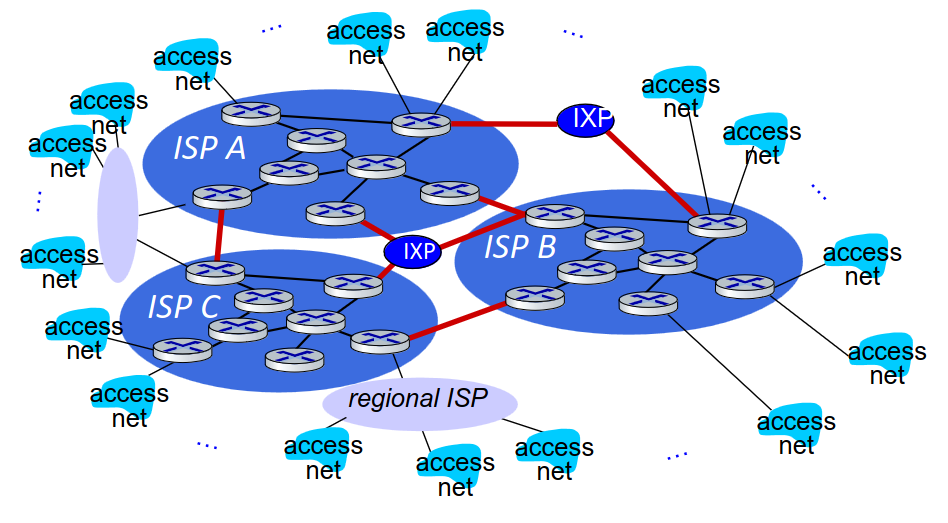
\includegraphics[scale=0.35]{Immagini/Rete-di-Reti.png}
        \caption{Struttura della rete Internet}
    \end{figure}
    

    \end{sloppypar}

\end{document}  